%
% FDY TEMPLATE for ANUAL REPORT
% ===================================================================
% Reviewer 1: ...
% Reviewer 2: ...
%===================================================================
\NeedsTeXFormat{LaTeX2e}
\documentclass[11pt,twoside,a4paper]{fdyartcl}
\usepackage[utf8]{inputenc}
\usepackage[T1]{fontenc}
\usepackage[ngerman,english]{babel} % selectlanguage wird nur dann gebraucht, wenn
                                    % mehrere Sprachen-packages verwendet werden,
                                    % das zuletzt angegebene package ist die aktive
                                    % Sprache, mit \selectlanguage kann umgeschaltet
                                    % werden
\usepackage[intoc]{nomencl} % zur Erstellung einer Nomenklatur
                                   % Die Option [intoc] sorgt dafuer,
                                   % dass die Nomenklatur im
                                   % Inhaltsverzeichnis eingetragen
                                   % wird. Aufruf mit:
                                   % makeindex Diss.nlo -s nomencl.ist -o Diss.nls
\usepackage{longtable}  % fuer tabellen, die evtl ueber Seiten
                        % umgebrochen werden muessen
\usepackage{graphicx}   % Stellt \includegraphics zur Verfuegung
\usepackage{parskip}    % Setzt parindent auf null und parskip auf
                        % einen angemessenen Wert
\usepackage{calc}       % Erlaubt, verschiedene Masse zu addieren
                        % z.B 1cm+2pt
\usepackage[a4paper,twoside,outer=2.2cm,inner=3cm,top=1.5cm,bottom=2.7cm,includehead]{geometry}
                                        % erheblich verbesserte
                                        % Papieranassung
\usepackage{setspace}   % Stellt \singlespacing, \onehalfspacing und
                        % \doublespacig zur Verfuegung
                        % erlaubt ausserdem die Verwendung der
                        % Umgebung \begin{spacing}{2.3}
\setstretch{1.05}       % minimal vergroesserter Zeilenabstand
\usepackage{amsmath}    % Stellt verschiedene Mathematik Operatoren
                        % und Befehle bereit und verbessert die
                        % Darstellung von Gleichungen ermoeglicht
                        % ausserdem die Verwendung von \boldsymbol
                        % fuer z.B. griechische Buchstaben
\usepackage{amsfonts}
\usepackage{amsthm}
\usepackage{harvard}    % neue citation Befehle und anderes Layout der
                        % Bibliographie
\usepackage{mathpazo}   % Aenderung der Standardschrift auf Palatino
\bibliographystyle{diss_harv_babel}
\input babelbst.tex     % sonst funktioniert das zweite \cite Kommando
                        % nicht, weil im harvardstyle \bbletal{}
                        % herausgeschrieben wird
%\usepackage{showkeys}   % Spaeter auskommentieren
\usepackage{upgreek}    % nicht-kursive grichische Buchstaben
\usepackage{fancyhdr}

\usepackage{ngerman}    %erlaubt auf allen Btriebssystemen die Eingabe der Umlaute als "a,"o,"u und "s mit dem Ergebnis
                        % ä,ö,ü und ß.(Gleiches gilt für Großbuchstaben)
\usepackage{listings}
\usepackage{subfig}
\usepackage{hyperref}
\usepackage{wsDBEtex}   %this is the style package to display .bws content

\graphicspath{{./Figures/}}%
% \input hyphen_dt.tex  % Spezielle Trennregeln fuer deutsche
                        % Woerter - gehoert in den Vorspann
\clubpenalty = 10000%
\widowpenalty = 10000%
\displaywidowpenalty =10000


%%%%%%%%%%%%%%%%%%%%%%%%%%%%%%%%%%%%%%%%%%%%%%%%%%%%%%%%%%%%%%%%%%%%%
%%%%%%%%%%%%%%%%%%%%%%%%%%%%%%%%%%%%%%%%%%%%%%%%%%%%%%%%%%%%%%%%%%%%%
% TITLE AND AUTHOR
%%%%%%%%%%%%%%%%%%%%%%%%%%%%%%%%%%%%%%%%%%%%%%%%%%%%%%%%%%%%%%%%%%%%%
%%%%%%%%%%%%%%%%%%%%%%%%%%%%%%%%%%%%%%%%%%%%%%%%%%%%%%%%%%%%%%%%%%%%%
\title{Guide for HHLR Cluster}
\author{Stephan Krämer-Eis, Björn Müller, revised by Dennis Krause, Markus Geisenhofer}
%%%%%%%%%%%%%%%%%%%%%%%%%%%%%%%%%%%%%%%%%%%%%%%%%%%%%%%%%%%%%%%%%%%%%
%%%%%%%%%%%%%%%%%%%%%%%%%%%%%%%%%%%%%%%%%%%%%%%%%%%%%%%%%%%%%%%%%%%%%
%%%%%%%%%%%%%%%%%%%%%%%%%%%%%%%%%%%%%%%%%%%%%%%%%%%%%%%%%%%%%%%%%%%%%

%%%%%%%%%%%%%%%%%%%%%%%%%%%%%%%%%%%%%%%%%%%%%%%%%%%%%%%%%%%%%%%%%%%%%
%%%%%%%%%%%%%%%%%%%%%%%%%%%%%%%%%%%%%%%%%%%%%%%%%%%%%%%%%%%%%%%%%%%%%
% Kopfzeile
\pagestyle{fancy}
\fancyhf{}
\renewcommand{\headrulewidth}{0pt}

%\fancyhead[CE]{\sffamily \normalsize \thepage \quad \hrulefill \quad \sffamily \normalsize Short Title of Your Report }
%\fancyhead[CO]{\sffamily \normalsize F. Kummer \quad \hrulefill \quad \sffamily \normalsize \thepage }
\fancyhead[CE]{\sffamily \small \thepage \quad \hrulefill \quad \sffamily \small Guide for HHLR Cluster }
\fancyhead[CO]{\sffamily \small FDY \quad \hrulefill \quad \sffamily \small \thepage }


%%%%%%%%%%%%%%%%%%%%%%%%%%%%%%%%%%%%%%%%%%%%%%%%%%%%%%%%%%%%%%%%%%%%%
%%%%%%%%%%%%%%%%%%%%%%%%%%%%%%%%%%%%%%%%%%%%%%%%%%%%%%%%%%%%%%%%%%%%%

% Angaben fuer die Nomenklatur
%\makenomenclature
%\renewcommand{\nomname}{Nomenklatur}
%\setlength{\nomitemsep}{-0.2\parsep}% Der Abstand zweier Eintraege in
                                    % der Nomeklatur betraegt

% Dieser Befehl stellt sicher, dass neue Kapitel auf rechten (ungeraden) Seiten beginnen
\newcommand{\clearemptydoublepage}%
{\newpage{\pagestyle{empty}\cleardoublepage}}
\newfont{\myrm}{cmr12 at 12 pt}
% FigureXYLabel - urspruenglich in defin.tex, von Prof.~Dr.-Ing.~M. Oberlack
% Urspruengliche Version umfasste 5 Parameter -  geaenderte 7 Parameter - Bauerbach
% 1 Figurename: \includegraphics[......
% 2 Beschriftung der x Achse
% 3 x-Beschriftung - Verruecken horizontal positiv nach links
% 4 x Beschriftung - Verruecken vertikal positiv nach unten
% 5 Beschriftung der y Achse
% 6 y-Beschriftung - Verruecken horizontal positiv nach links
% 7 y Beschriftung - Verruecken vertikal positiv nach oben
\newlength{\FigureHeight}
\newlength{\FigureHeightHalf}
\newcommand{\FigureXYLabel}[7]{%
\settoheight{\FigureHeight}{#1}%
\setlength{\FigureHeightHalf}{0.5\FigureHeight}%
\addtolength{\FigureHeightHalf}{#7}%
\raisebox{\FigureHeightHalf}{\makebox[0cm][r]{#5\makebox[#6]{}}}%
#1\\%
\vspace{#4}%
{\makebox{#2\makebox[#3]{}}}}
%
%%%%%%%%%%%%%%%%%%%%%%%%%%%%%%%%%%%%%%%%%%%%%%%%%%%%%%%%%%%%%%%%%%%%%
%\addtokomafont{sectioning}{\rmfamily}
%\addtokomafont{section}{\normalsize}
%\addtokomafont{subsection}{\normalsize}

\newcommand{\Bosss}{\textit{BoSSS}}

%\usepackage{sectsty}
%\sectionfont{ \parskip=0mm \vspace*{-5mm} }
%\subsectionfont{ \parskip=0pt \vspace*{-1mm} \centering \normalfont \normalsize \itshape}
%\paragraphfont{ \normalfont \itshape }

%% this is for showing a content of a .json-file
\usepackage{listings}
\usepackage{xcolor}

\colorlet{punct}{black}
\colorlet{delim}{black}
\colorlet{numb}{black}

\lstdefinelanguage{json}{
	basicstyle=\normalfont\ttfamily,
	numbers=left,
	numberstyle=\scriptsize*,
	stepnumber=1,
	numbersep=8pt,
	showstringspaces=false,
	breaklines=true,
	frame=lines,
	literate=
%	*{0}{{{\color{numb}0}}}{1}
%	{1}{{{\color{numb}1}}}{1}
%	{2}{{{\color{numb}2}}}{1}
%	{3}{{{\color{numb}3}}}{1}
%	{4}{{{\color{numb}4}}}{1}
%	{5}{{{\color{numb}5}}}{1}
%	{6}{{{\color{numb}6}}}{1}
%	{7}{{{\color{numb}7}}}{1}
%	{8}{{{\color{numb}8}}}{1}
%	{9}{{{\color{numb}9}}}{1}
	{:}{{{\color{punct}{:}}}}{1}
	{,}{{{\color{punct}{,}}}}{1}
	{\{}{{{\color{delim}{\{}}}}{1}
	{\}}{{{\color{delim}{\}}}}}{1}
	{[}{{{\color{delim}{[}}}}{1}
	{]}{{{\color{delim}{]}}}}{1},
}


%       DOKUMENT
\begin{document}

\pagenumbering{arabic} % Zurueckschalten auf arabische Ziffern, dabei wird der Zaehler auf 1 gesetzt

%%%%%%%%%%%%%%%%%%%%%%%%%%%%%%%%%%%%%%%%%%%%%%%%%%%%%%%%%%%%%%%%%%%%%%%%%%%%%%%%55
% Seitennummer der ersten Seite
\setcounter{page}{1} % must be an odd number
                       % muss eine ungerade Zahl sein
%%%%%%%%%%%%%%%%%%%%%%%%%%%%%%%%%%%%%%%%%%%%%%%%%%%%%%%%%%%%%%%%%%%%%%%%%%%%%%%%55
%%%%%%%%%%%%%%%%%%%%%%%%%%%%%%%%%%%%%%%%%%%%%%%%%%%%%%%%%%%%%%%%%%%%%%%%%%%%%%%%55
%%%%%%%%%%%%%%%%%%%%%%%%%%%%%%%%%%%%%%%%%%%%%%%%%%%%%%%%%%%%%%%%%%%%%%%%%%%%%%%%55

% Titelseite
% -------------------
\maketitle


\begin{abstract}
%\textbf{Abstract:}
This best practice guide gives an overview over the required steps to run BoSSS on the HHLR cluster. It gives some informations about the cluster itself and starts with a step by step tutorial how to install the necessary libraries on the cluster. Furthermore a commented batch script is given to run a \Bosss application on the compute nodes.
\end{abstract}




%==================== Hauptteil =====================================
%
\section{Notation}
\label{sec:notation}
\begin{description}
	\item[\$executable] arbitrary executable within BoSSS framework compiled on your local machine
	\item[\$executablePath] The path to the executable on your local machine, which you want to execute on the cluster
	\item[\$BosssDir] directory to your \Bosss repository on your local machine
	\item[\$BoSSSInstallDir] directory of recent \Bosss installation on your local machine
	\item[\$BoSSSNetDrive] the \Bosss network drive reachable over \verb|\\dc1\bosss\| (mount that drive!)
	\item[\$TuID] Your TU-ID
	\item[\$home] Your home directory on the cluster
	\item[\$deployDir] An arbitrary sub-directory of \verb|$home| to which the executables will be deployed
	\item[\$databaseDir] The location of a \Bosss database on the cluster, which might be not a sub-directory of \verb|$home| (usually root:/work/scratch/\verb|$TuID|)
	\item[\$host] The host name of one of the login nodes of the cluster. Currently, you can select e.g. lcluster2.hrz.tu-darmstadt.de, or lcluster8.hrz.tu-darmstadt.de
\end{description}

\section{General information about the cluster}
\label{sec:information}

The HHLR Lichtenberg cluster consists of 780 compute nodes and 4 login nodes. The cluster is split into 3 sections: 
\begin{itemize}
	\item MPI, for communication (MPI) intensive applications
	\item MEM, for memory intensive applications
	\item ACC, for applications which are using accelerators, like GPU computations
\end{itemize}
note: The 'AVX2'-nodes are selected by \Bosss as default, which correspond to the MPI section. In order to use another section, you have to modify the deployed bash sheet.
%The compute nodes are subdivided into 19 islands: 17 island with each 32 nodes (512 cores), 1 island with 160 nodes (2560 cores) and 1 island with accelerator nodes (CUDA cores and Xeon Phi Coprocessors). For \Bosss applications the MPI section is most suitable, to which the 17 islands and the island with 160 nodes belong. Each of this nodes consists of 2 processors with 8 cores (in total 16 cores per node) and 32 GB memory.\\

\begin{itemize}
\item Phase I (Lichtenberg II): 604 nodes (login: 8, MPI: 596, MEM: 4, ACC: 32)
\item Phase I (Lichtenberg I): decommissioned
\item Phase II (Lichtenberg I): 640 nodes (login: 8, MPI: 586, MEM: 2, ACC: 8)
\end{itemize}
(state 20.07.2020.)

Check \ \url{https://www.hhlr.tu-darmstadt.de/hhlr/betrieb/hardware$\_$hlr/index.de.jsp} for the detailed hardware specifications.

The file system is divided into 3 sections:
\begin{itemize}
\item \verb|/home|: With your application for an account, you get your home directory which you can find under \verb|/home/$TuID|. This directory can be accessed from all nodes and has a daily backup of your data. The quota is limited to 15 GB. 
\item \verb|/work/local|: These are the local hard drives of the node and can only be accessed from the particular node. Attention: After a job has finished, all data will be erased! 
\item \verb|/work/scratch|:  This directory can be accessed from all nodes. With your application, there will be the folder \verb|/work/scratch/$TuID|. You have unlimited quota, but all data is erased after 30 days without any warning! 
\end{itemize}
More information: \\ \url{https://www.hhlr.tu-darmstadt.de/hhlr/arbeit_auf_dem_cluster/dateisysteme_lichtenbergrechner_2/index.de.jsp}


\section{Installation on the cluster}

The HHLR cluster provides some preinstalled libraries, like \verb|openmpi| or \verb|matlab|. The command \verb|module available|  lists them all. This is the configuration, which has proved to be functional for the recent code (state 20.07.2020):
\begin{table}[h]
	\centering
	\begin{tabular}{l|c}
		gcc & 8.3.0 \\
		cmake & 3.17.1 \\
		openucx & 1.7.0 \\
		mono & 6.0.0 \\
		openblas & 0.2.20 \\
		openmpi & 4.0.3
	\end{tabular}
\end{table}
The Linux C\# compiler \emph{mono} is provided by the platform and must not be installed by hand. There are two ways to install the libraries:
\begin{itemize}
	\item (recommended) Copy the binaries from your local \Bosss-Installation onto the cluster and have fun
	\item Download the latest version from the developers homepage and install them manually 
\end{itemize}

These libraries, which are distributed by the \Bosss-installation, will be called \Bosss-native libraries subsequently.
The binary for \emph{ParMETIS} and \emph{Hypre} are not distributed with the \Bosss-native libraries. You can copy them from \verb|$BoSSSNetDrive|. Simply follow the steps in section \ref{sec:putty}, \ref{sec:bashconfig} and \ref{sec:copylibs}.

The manual installation is not recommended for the inexperienced user, since you can encounter problems during compilation and execution of the binaries, due to version incompatibility with the \Bosss-code or other libraries.
For details you can check the bash scripts of the \Bosss-native.git online repository (url:\url{https://github.com/FDYdarmstadt/BoSSS-native.git}). This repository is used to build and test libraries, which are used with the recent source code.
Older instructions can be found in folder 'old instructions'.

\subsection{Connecting to the cluster}
\label{sec:putty}
In general, the \emph{ssh} protocol is used to access the cluster. An \emph{ssh} connection can be established by simply using the \emph{ssh} command on the console (see the following section), but more sophisticated tools exist that allow for a simpler configuration of advanced connection settings. On Windows machines, the program \emph{PuTTY} is used predominantly, and this tutorial will briefly demonstrate its usage in section \ref{sec:dbe}. It should be noted, however, that \emph{PuTTY} is nothing but a graphical wrapper around the plain \emph{ssh} which means that all options can be used on the console, too.

\subsection{configure .bashrc}
\label{sec:bashconfig}
The \textit{bashrc} allows you to configure your bash you are using on the cluster. It is located in your home directory, which you enter by login. You can access its content via a text editor e.g. nano. Now we specify, which libraries provided by the platform, shall be loaded.
\begin{enumerate}
	\item insert these lines into your \textit{bashrc} with a text editor of your choice (e.g. prompt \verb|nano .bashrc|):
	\begin{verbatim}
	module load git
	module load gcc
	module load mono
	module load openblas/0.2.20
	module load openmpi
	\end{verbatim}
	
	\item Save these changes and close the texteditor (e.g. with \verb|Ctrl + X| when using nano). Do not forget to update your bash afterwards by prompting:
	\begin{verbatim}
	source .bashrc
	\end{verbatim}
\end{enumerate}


\subsection{Copy libraries}
\label{sec:copylibs}
The native libraries are distributed via the \Bosss-installation on your local machine. You just have to navigate to and copy the libraries for linux onto the cluster. The native libraries include:

\begin{table}[h]
	\centering
	\begin{tabular}{l|c|c}
		name & vendor & parallelism \\
		\hline
		BLAS(MKL) & Intel & SEQ \\
		LAPACK(MKL) & Intel & SEQ \\
		TECIO & Tecplot, Inc. & SEQ \\
		MUMPS & many & SEQ, MPI \\
		PARDISO(MKL) & Intel & SEQ, OpenMP \\
		METIS & karypis labs & SEQ
	\end{tabular}
\end{table}



\begin{enumerate}
	\item Goto \ \url{https://github.com/FDYdarmstadt/BoSSS/releases} \ download and install the latest release on your local machine. \verb|$BoSSSInstallDir| will be the path you specify during installation. You can check it by prompting \verb|echo %BOSSS_INSTALL%| in cmd or \verb|echo $BOSSS_INSTALL| in shell/bash. \\
	NOTE: Also use the latest version of the \Bosss code. If you intend to use an older version, make sure you have installed the corresponding release.
	\item navigate to the linux libraries, by prompting:
	\begin{verbatim}
		cd $BoSSSInstallDir\bin\native\linux\amd64-openmpi
	\end{verbatim}
	\item copy all the containing .so-libraries to your \verb|$home| directory:
	\begin{verbatim}
		scp *.so $TuID@$host:.
	\end{verbatim}
	REMARK: you will notice, that the \textit{.bashrc} is executed during this command.
	\item login to the cluster:
	\begin{verbatim}
		ssh $TuID@$host
	\end{verbatim}
	\item give the libraries a directory, that they have it warm and save:
	\begin{verbatim}
		mkdir bosss_install
		cp *.so bosss_install
	\end{verbatim}
	\item Now we have to make the information, where these libraries are located, available for \Bosss. Therefore we set an environment variable. Insert this line into your \textit{bashrc}, with a text editor of your choice (e.g. prompt \verb|nano .bashrc|):
	\begin{verbatim}
	 	export BOSSS_INSTALL=/home/$TuID/bosss_install
	\end{verbatim}
	close editor and save changes to your \textit{bashrc} (e.g. with \verb|Ctrl + X| when using nano)
	\item update your bash afterwards by prompting:
	\begin{verbatim}
		source .bashrc
	\end{verbatim}
\end{enumerate}
REMARK: For now you have to imitate the relative path to the libraries within the \verb|$BoSSSInstallDir| on your local machine, that \Bosss is able to find the libraries: you have to put the libraries here \verb|bosss_install/bin/native/linux/amd64-openmpi| instead of \verb|bosss_install|.

The libraries of \emph{Hypre} and \emph{ParMETIS} are not essential for \Bosss at the moment.
\emph{ParMETIS} is a MPI-parallel version of \emph{METIS}. \emph{METIS} and \emph{ParMETIS} are used for grid partitioning in \Bosss. In Practice the partitioning is not very time consuming in comparison to other methods. So \emph{METIS} is probably sufficient for small and medium scale parallelism.
\emph{Hypre} is not used by \Bosss at the moment. (state 29.07.2020).
If do not have the urgent need to use these libraries, you can skip subsequent steps.

\begin{enumerate}
	\item navigate to the network drive \verb|\\dc1\bosss\binaries\hhlr\|
	\item copy the necessary .so-libraries to your \verb|$home| directory:
	\begin{verbatim}
	scp ParMETIS/libparmetis.so $TuID@$host:$bosss_install_linux
	scp Hypre/hypre-2.9.0b_bin/lib/libHYPRE.so $TuID@$host:$bosss_install_linux
	\end{verbatim}
	where \verb|$bosss_install_linux| is the path, where you copied the native libraries.
	\item proceed to testing plz
\end{enumerate}


\subsection{Testing the libraries}
\label{sec:testing}
All necessary libraries are installed on the cluster. Now we can test them by running a small \Bosss application. As test problem, we choose the ipPoisson problem. In this particular case we run the problem directly on the login node, because it takes only a few seconds to compute. 

In general: Never run a computation on a login node! How to run a computational heavy application is explained later in section \ref{sec:WorkingHHLR}.

%\textbf{Important note about the console application you use:} If you use \emph{git bash}, you should consider using another one (at least for this case). As \emph{git bash} is based on a console named \emph{mintty} which Windows recognizes as a normal program and not as a console application, there will be problems when entering your password for the Lichtenberg cluster, without going into too much detail. Alternatives are other console applications, such as \emph{cmd}, \emph{powershell} or \emph{ConEmu}. The last mentioned one is quite popular at FDY.

This is a brief test, which tests if the native libraries can be loaded and also tries to execute some methods of these libraries.
Because \emph{gitbash} is used by most people at fdy, the steps are considered to be prompted in \emph{gitbash}. The commands may vary for other consoles.
\begin{enumerate}
	\item deploy the \emph{BoSSSpad} with its dependencies to the cluster:
	\begin{verbatim}
		cd $BOSSS_INSTALL/bin/Release
		./bcl deploy-at BoSSSpad.exe sftp://$TuID@$host:BoSSSpad
	\end{verbatim}
	\item login onto cluster:
	\begin{verbatim}
		ssh $TuID@$host
	\end{verbatim}
	\item perform a test of loading dependencies:
	\begin{verbatim}
		mono BoSSSpad/BoSSSpad.exe --check
	\end{verbatim}
	\item there will be a short summary, which libraries could be loaded.
\end{enumerate}
In this case \verb|BoSSSpad/| is the \verb|$deployDir|, \verb|BoSSSpad.exe| the \verb|$executable| and \verb|$BOSSS_INSTALL/bin/Release/BoSSSpad.exe| the \verb|$executablePath|.
REMARK: refer to \verb|mono BoSSSpad/BoSSSpad.exe --help| to see more options of \emph{BoSSSpad}

Now we test if the libraries are functional, which should be the case except you compiled them on your own - you daredevil!
\begin{enumerate}
\item compile the ipPoisson project (in src/public/L4-applications/ipPoisson) on your local machine, e.g in Visual Studio
\item transfer the application and its dependencies to the cluster by using the \verb|bcl deploy-at| command with \verb|$executablePath=$BosssDir/src/public/L4-application/ipPoisson/bin/Release/ipPoisson.exe|, we will choose \verb|$deployDir=ipPoisson| 
\begin{verbatim}
$BOSSS_INSTALL/bin/Release/bcl deploy-at $executablePath sftp://$TuID@$host:ipPoisson
\end{verbatim}
\item \verb|bcl deploy-at| only copies the application but not a control file. Copy a suitable control file by using \verb|scp|
\begin{verbatim}
scp control-example.xml $TuID@$host:ipPoisson
\end{verbatim}
\item login on the cluster
\begin{verbatim}
ssh $TuID@$host
\end{verbatim}
\item now the program can be started
\begin{verbatim}
cd ipPoisson
mono ipPoisson.exe --control control-example.xml
\end{verbatim}
\item if everything is working, the program should be end with \verb|converged? true|. Then a parallel run on two cores can be tested:
\begin{verbatim}
mpiexec -n 2 mono ipPoisson.exe --control control-example.xml
\end{verbatim} 
\end{enumerate}
If both tests run, the installation of \Bosss on the HHLR cluster was successful.

\section{Setup and synchronization of the \Bosss database}
\label{sec:BoSSSdb}
For most of the \Bosss applications you need a database (db). Since you cannot use the graphical Database Explorer on the cluster, you need to synchronize your db on your local machine in order to evaluate your results. Databases can be created manually (see section \ref{sec:setup_db}). But we recommend to mount the relevant drives to your machine, than you can access and manage your databases easily with your local \emph{BoSSSpad} (see section \ref{sec:mountonwindows}).
If your scratch direcory is mounted, you can copy and paste files as usual. But for larger databases or if you want to customize synchronization you can use for example \emph{WinSCP} (see section \ref{sec:synchronize_db}).

\subsection{Mount drives to windows 10}
\label{sec:mountonwindows}
This approach is relatively stable, but acquires some software to be installed: WinFSP is combinded with SSHFS-Win.

\begin{enumerate}
	\item follow the instructions at \url{https://github.com/billziss-gh/winfsp/releases} to install WinFSP
	\item follow the instructions at \url{https://github.com/billziss-gh/sshfs-win/releases} to install SSHFS for windows
	\item after you installed the software, you can mount every path you want of the cluster onto your local machine.
	Open the \emph{file explorer} and rightclick on the 'this PC' node, select 'map networkdrive ...'
	%\begin{figure}[htbp] % htb: preferred position of picture: here, top, bottom of page
	%\begin{centering}
	%\includegraphics[width=0.9\textwidth]{Figures/mapdrive.png}\\
	%\end{centering}
	%\caption{map drive - open dialogue}\label{fig:map_drive}
	%\end{figure} %
	\item choose a drive letter in the new dialogue, set the checkbox 'Reconnect at sign-in'
		\begin{figure}[htbp] % htb: preferred position of picture: here, top, bottom of page
		\begin{centering}
		\fbox{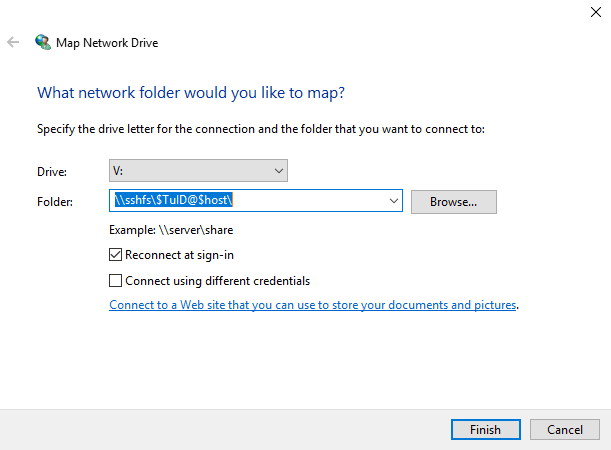
\includegraphics[width=0.75\textwidth]{Figures/mapdrive_2.png}}\\
		\end{centering}
		\caption{map drive - fill dialogue}\label{fig:map_drive_dia}
		\end{figure} %
	\item now fill the field 'Folder:' with
	\begin{verbatim}
		\\sshfs\$TuID@$host\
	\end{verbatim}
	Close dialogue by clicking 'Finish'. Now you are prompted to confirm the connection with your password (same as for cluster login)
	\item the mapped drive now should appear in your \emph{file explorer}
\end{enumerate}
Other useful paths to map are e.g.
\begin{itemize}
	\item[] scratch-folder: \verb|\\sshfs\$TuID@$host\..\..\scratch\$TuID|
	\item[] root of cluster file system: \verb|\\sshfs\$TuID@$host\..\..\|
	(type \verb|\\sshfs\\$TuID@$host\\..\\..\\..| to do so)
\end{itemize}

Now you shall be able to use the mounted drives as any other drive on your system. For example you can access a database via \emph{BoSSSpad} with \verb|OpenOrCreateDatabase(@"$DBpath")|. A brief introduction is given in section \ref{sec:bla}. Please see the tutorials within the \Bosss-handbook for further details.

\subsection{Synchronizing databases}
\label{sec:synchronize_db}
There are many ways to synchronize the db. An easy way is to use the tool \emph{WinSCP}. First you have to enter your login data, shown in figure \ref{fig:winscp_login}.
\begin{figure}[h] % htb: preferred position of picture: here, top, bottom of page
  \begin{centering}
  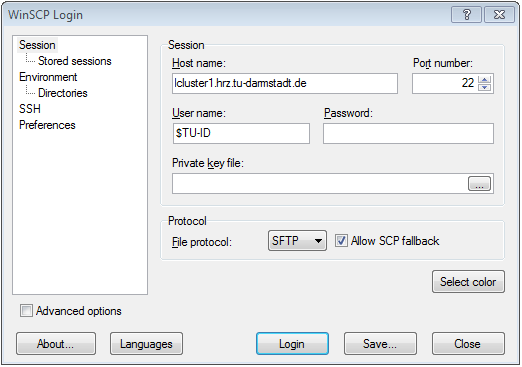
\includegraphics[width=0.9\textwidth]{Figures/winscp_login.png}\\
  \end{centering}
  \caption{WinSCP - Login data}\label{fig:winscp_login}
\end{figure} %
After logging in, you see on the left side your local file system and on the right side is your \verb|$home| directory on the cluster. Browse in both windows to the generated db (according to section \ref{sec:setup_db} this would be \verb|c:\BoSSS_db| on your local machine and \verb|/home/$TuID/BoSSS_db| on the cluster). \emph{WinSCP} has a build in synchronization tool, which is indicated with a red circle in figure \ref{fig:winscp_sync}.
\begin{figure}[t] % htb: preferred position of picture: here, top, bottom of page
  \begin{centering}
  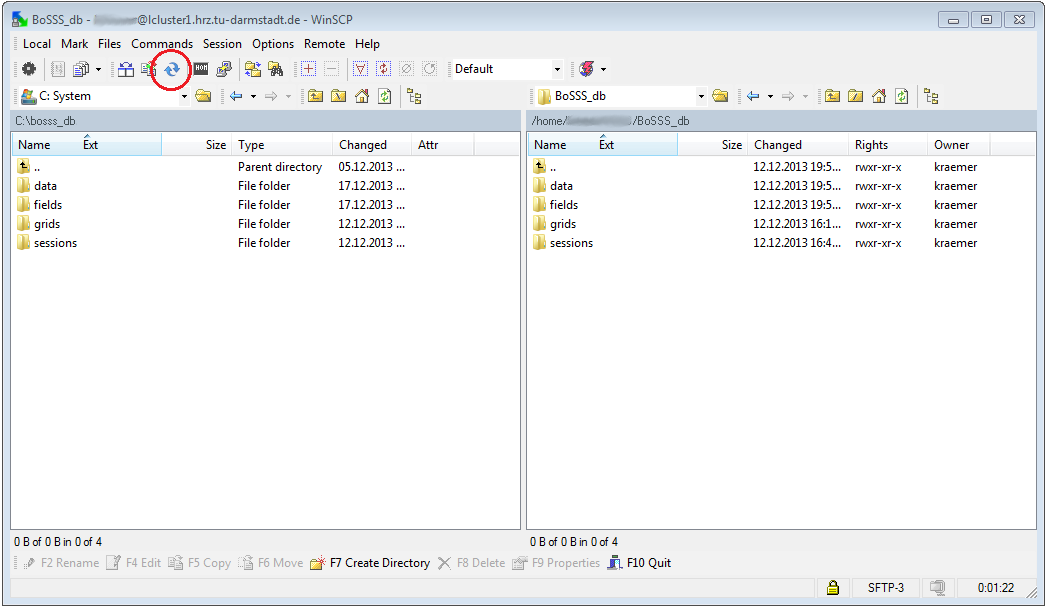
\includegraphics[width=0.9\textwidth]{Figures/winscp_sync.png}\\
  \end{centering}
  \caption{WinSCP - Synchronization}\label{fig:winscp_sync}
\end{figure} %
For the synchronization you have different options, e.g. from local to remote, from remote to local or in both directions.
You can also copy single files per drag and drop between both windows.

\subsection{Setting up a database manually}
\label{sec:setup_db}
You can create a dabatase manually and copy it the cluster by following these steps:
\begin{enumerate}
	\item create locally a new folder for your db, e.g. \verb|c:\BoSSS_db|
	\item open git bash and go to the folder, then prompt
	\begin{verbatim}
	bcl init-db
	\end{verbatim}
	\item now you have created a new db locally. By using \verb|scp| you can copy it to the cluster:
	\begin{verbatim}
	scp -r /c/BoSSS_db/ $TuID@$host:~/
	\end{verbatim}
\end{enumerate}

\subsection{Tips and Tricks}
\label{sec:tips}
\begin{itemize}
\item As mentioned in section \ref{sec:information} you have a quota of 15 GB in your home directory. If your planning big and/or many simulations, you might exceed this limit. Instead of using your \verb|$home| directory, you can use \verb|/work/scratch/$TuID| for your db. It has the advantage that you have nearly unlimited quota and \verb|/work/scratch| is a faster file system, i.e. less time is needed to save each timestep. But be careful: You have to take care of the data. On \verb|/work/scratch| data is deleted after 30 days without any warning!
\item If you have big databases and want them to synchronize only in one direction, e.g from the cluster on your local machine, it can take some time. Reason is that \Bosss saves every field in each timestep in a single file, hence you have lots of small files to copy. It can be faster to put the whole db in one archive and then just copy the archive to your local machine.
\end{itemize}


\section{Working on the HHLR Cluster}
\label{sec:WorkingHHLR}
We just pointed out that the login nodes are only intended to access the cluster, to copy data and to prepare/submit jobs. Do not start any computation on the login nodes! \\
You can deploy jobs directly with your \emph{BoSSSpad}, this will be shown in section \ref{sec:}.
When the binaries are deployed at the cluster a batch script is needed to specify the job parameters, like number of cores or memory allocation per core and stuff. The content of the batch script is detailed in section \ref{sec:}.
At least a completely workflow is described (section \ref{sec:}), how you can deploy and submit a job by hand. You rarely need to do this by hand, leave the deployment and submission to \emph{BoSSSpad}. Refer to this section rather as look behind the scene.

\subsection{Using \emph{BoSSSpad} for job submission}
\label{sec:BoSSSpad}

If you succeeded in mounting the \verb|scratch\$TuID| directory, there is no need for forwarding graphical output etc. As mentioned, you can use your local \emph{BoSSSpad} to manage databeses on the cluster as they would be on your local machine. In this section the process of deploying jobs completely via \emph{BoSSSpad} is shown. To do so some preparation is needed.

The configuration of \emph{BoSSSpad} is determined with some files located at \verb|C:\Users\$username\.BoSSS\etc|:
\begin{itemize}
	\item[] \textbf{DBE.xml} sets the standard databases, which are available right after the \verb|restart| command in \emph{BoSSSpad}
	\item[] \textbf{BatchProcessorConfig.json} configures the clients, which handle the connection to and the job submission to several servers, for example the HPC (at the fdy chair) or the HHLR cluster. 
\end{itemize}

To set the standard database with \verb|DBE.xml| is not mandatory and thus skipped.
To make your own Please refer to the examples in the attached \verb|sample| folder.
In \ref{lst:bpc} you can find the content of a BatchProcessorConfig.json with placeholders.


\noindent
\begin{minipage}{\linewidth}
\begin{lstlisting}[caption={example of BatchProcessorConfig.json}, label={lst:bpc} ,language=json,firstnumber=1]
{
 "AllQueues": [
  {
   "$type": "BoSSS.Application.BoSSSpad.SlurmClient, BoSSSpad",
   "Username": "$TuID",
   "ServerName": "$host",
   "PrivateKeyFilePath": "C:\\Users\\$Username\\.ssh\\id_rsa",
   "DeploymentBaseDirectory": "C:\\standard_deploy_dir",
   "DeployRuntime": false,
   "AllowedDatabasesPaths": ,
   "SlurmAccount": "project12345",
   "DeploymentBaseDirectoryAtRemote": "/home/$TuID/deploy_dir_at_HHLR"
  }
 ]
}
\end{lstlisting}
\end{minipage}
where \verb|$Username| is your account name within the FDY-domain.\\
NOTE: \$type is not a placeholder here!
\begin{itemize}
	\item[] \textbf{PrivateKeyFilePath} field is the path to your private ssh-key saved in RSA-Format.
	With these key pairs (private on your local machine, public at the server) you do not need to login with your password at the cluster anymore.
	This makes things easier, but is not mandatory. 
	\item[] \textbf{DeploymentBaseDirectory} is the default deploy directory at your local machine
	\item[] \textbf{AllowedDatabasesPaths} restricts the usage of databases to the bases you list here, you can leave this blank
	\item[] \textbf{SlurmAccount} your main projectId
	\item[] \textbf{DeploymentBaseDirectoryAtRemote} default deploy directory at the cluster
\end{itemize}

After you created/configured your BatchProcessorConfig.json, we can proceed with the submission workflow via \emph{BoSSSpad}.
In our example \emph{BoSSSpad} worksheet (filetype .bws), which is shown in listing \ref{lst:bps}, we will submit a job, which is solving the SIP discretized Poisson problem.
Please note that this example contains placeholders, it is not copy-paste-execution ready.
You have to configure it for your usage.
The \verb|restart| e.g. loads all databases, which are listed in DBE.xml.
\verb|ExecutionQueques| will list all clients, which are configured in the BatchProcessorConfig.json, which is the one of \ref{lst:bpc} in our case.
In line 3 the object \verb|myBatch| is instanced as SlurmClient type.
We will use it later to finally submit the job.
In the next paragraph (line 4 to 6) we load a database 'test\_DB', the drive 'W' is the mounted 'root' of the cluster.
After the database is loaded, it can be handled as any other database on your local machine.
The using directive in line 7 is for comfort. Otherwise you would have to type the full namespace dependencies everytime.
Now we create the control object, which is of type 'SipControl' in this case.
Lines 11 to 13 are important, there the path to the database is specified.
Line 12 is the path on the cluster and line 13 is the path on your local machine.
At execution these paths are tested to be existent.
The one, who is, will be selected for saving the database.
In addition you can specify a machine filter (second string).
If a filter is specified only the paths are tested, where the filter matches the machine name.
This is only a fragment of the control object configuration, grid, boundary conditions, etc. are left out for simplification.
In the last paragraph the job is configured.
The job attributes are basically the corresponding flags of the batch script, which are detailed in section \ref{sec:sbatch}.
In line 15 the type of the executable is overgiven, that all dependant libraries can be determined for deployment on the cluster. 
With \verb|aJob.Activate(myBatch)| the binaries are deployed and the job is quequed by the scheduler of the cluster. 

\noindent
\begin{minipage}{\linewidth}
	\begin{lstlisting}[caption={example of Job Submission via BoSSSpad}, label={lst:bps}]
	\end{lstlisting}
	\BoSSScmd{
restart
 }
\BoSSSexeSilent
\BoSSScmd{
ExecutionQueues;
 }
\BoSSSexe
\BoSSScmd{
var myBatch = (SlurmClient)ExecutionQueues[0];
 }
\BoSSSexe
\BoSSScmd{
string path = @"W:\textbackslash work\textbackslash scratch\textbackslash TuID\textbackslash test\_DB";\newline 
var tempDB  = OpenOrCreateDatabase(path);\newline 
tempDB.Sessions;
 }
\BoSSSexe
\BoSSScmd{
using BoSSS.Application.SipPoisson;
 }
\BoSSSexe
\BoSSScmd{
var ctrl         = new SipControl();\newline 
ctrl.savetodb    = true;\newline 
ctrl.SessionName = "SIP\_test";\newline 
ctrl.AlternateDbPaths = new[]\{\newline 
\btab \btab new ValueTuple<string,string>(@"/work/scratch/TuID/test\_DB", ""),\newline 
\btab \btab new ValueTuple<string,string>(@"W:\textbackslash work\textbackslash scratch\textbackslash TuID\textbackslash test\_DB", "")\newline 
\btab \};
 }
\BoSSSexe
\BoSSScmd{
var aJob = new Job(ctrl.SessionName, typeof(SipPoissonMain));\newline 
aJob.SetControlObject(ctrl);\newline 
((SlurmClient)ExecutionQueues[1]).SlurmAccount = "project12345";\newline 
aJob.NumberOfMPIProcs         = 2;\newline 
aJob.ExecutionTime            = "01:00:00";\newline 
aJob.HHLR\_project             = "project12345";\newline 
aJob.MemPerCPU                = "5000";\newline 
aJob.UseComputeNodesExclusive = true;\newline 
aJob.Activate(myBatch);
 }
\BoSSSexe

	%\renewcommand{\BoSSSbwsName}{UsingSlurmClient}
	
\end{minipage}

%\begin{lstlisting}[caption={Submission over Startup string}, label={lst:bps_ws}]
%\end{lstlisting}
%\setcounter{BoSSSblkCounter}{-1}
%\setcounter{BoSSSinblkCounter}{-1}
%\renewcommand{\BoSSSbwsName}{UsingSlurmClientStartupString}
%
%\BoSSScmd{
string StartupString = string.Format("cs:BoSSS.Application.SipPoisson.SipHardcodedControl.TestCartesian1(\{0\},\{1\},\{2\},\{3\},\{4\})", 32, 1.0, 16, 1.01, 2);
 }
\BoSSSexeSilent
\BoSSScmd{
var aJob = new Job(ctrl.SessionName, typeof(SipPoissonMain));\newline 
oneJob.SetCommandLineArguments(StartupString);\newline 
((SlurmClient)ExecutionQueues[1]).SlurmAccount = "project12345";\newline 
aJob.NumberOfMPIProcs         = 2;\newline 
aJob.ExecutionTime            = "01:00:00";\newline 
aJob.HHLR\_project             = "project12345";\newline 
aJob.MemPerCPU                = "5000";\newline 
aJob.UseComputeNodesExclusive = true;\newline 
aJob.Activate(myBatch);
 }
\BoSSSexeSilent


If you are not able to create a control object, which is not serializeable, e.g. because of Function delegates, there is another option.
If you create your control object from source code, you can use a startup string instead:

\lstinputlisting[basicstyle=\footnotesize\ttfamily\color{darkblue}, language=C, keywordstyle=\color{darkgreen}, stringstyle=\color{darkgrey}, commentstyle=\color{lightergray}]{UsingSlurmClientStartupString/in0-0.txt}

The starup string will replace line 8 to 14 of \ref{lst:bps}. This startup string is overgiven to the client by:

\lstinputlisting[basicstyle=\footnotesize\ttfamily\color{darkblue}, language=C, keywordstyle=\color{darkgreen}, stringstyle=\color{darkgrey}, commentstyle=\color{lightergray}]{UsingSlurmClientStartupString/in1-0.txt}

which replaces line 16 of \ref{lst:bps}.

\subsection{create private key for ssh}
\label{sec:sshkey}

You may want or need to create a private/public keypair for your ssh connections. The server checks if the client, which attempts to establish a connection, is in possession of a matching private key. If this turns out true, the connection is established, without an authentication from the user (password prompt). You can find plenty tutorials how to do this, so we stick to the basics here.

\begin{enumerate}
	\item open a ssh-capable bash/shell and start key generation by prompting:
	\begin{verbatim}
		ssh-keygen -m PEM -t rsa -b 4096
	\end{verbatim}
	\verb|ssh-keygen| should be sufficient, but with newer version an OPEN-SSH key is created by default, which is not supported by our implemented client.
	So we have to force the creation of an rsa key.
	You can check this by opening the .rsa file: the header should read 'BEGIN RSA PRIVATE KEY'.
	A dialogue will follow.
	\item the private key will be created in a path like \verb|C:\users\$username\.ssh\id_rsa| (linux: \verb|/home/username/.ssh/id_rsa|). If you created already a key, you are aksed, if you want to overwrite it. \\ NOTE: If you choose to overwrite the key on disk, you will not be able to authenticate using the previous key anymore.
	\item You can enter a passphrase for your keys or leave it empty (press enter). Consider this as a master key to all your connections.
	
	\item Now you have to copy the public key to the server:
	\begin{verbatim}
		ssh-copy-id $TuID@$host
	\end{verbatim}
\end{enumerate}



\subsection{the batch-script}
\label{sec:sbatch}

The HHLR cluster uses the SLURM batch system, which calculates when and on which node the job can be started. The nodes executes the batch-script line by line. The script consists of two parts: a ``Head'' part where all informations for the SLURM system are specified and a ``body'' where the commands are listed.\\

\noindent
\begin{minipage}{\linewidth}
\begin{lstlisting}[caption={Batch-script: head}, 
label={lst:head_batch}]
#!/bin/sh
# Job name
#SBATCH -J $job-name
#
# File / path where STDOUT will be written, the %J is the job id
#SBATCH -o /home/$TuID/$deployDir/$job-name.out%J
#
# File / path where STDERR will be written, the %J is the job id
#SBATCH -e /home/$TuID/$deployDir/$job-name.err%J
#
# Request the time you need for execution in minutes
# The format for the parameter is: [days:][hour:]minute,
# that means for 80 minutes you could also use this: 1:20
#SBATCH -t 23:59:59
#
# Request virtual memory you need for your job in MB per CPU
# 1750 MB is the maximum per core to run CPU efficient. If you
# use more, then not all CPU on a node can run!
#SBATCH --mem-per-cpu=1750
#
# Request the number of compute slots you want to use
#SBATCH -n 16
#
# Specify your mail address - for activation replace < your email> and remove prepending "# "
#SBATCH --mail-user=$yourName@fdy.tu-darmstadt.de
#
# Send a mail when job is done - for activation remove prepending "# "
#SBATCH --mail-type=END
#
#SBATCH -C avx
#SBATCH --exclusive
\end{lstlisting}

\end{minipage}

notes:
\begin{itemize}
	\item[] \textbf{execution-time:} your place in the queque is influenced by the execution time you reserved. Use an execution time below \verb|-t 1:00| to have your job running as soon as possible.
	\item[] \textbf{memory-per-cpu} be careful with the memory-per-cpu flag. This determines how much notes you are reserving. Example: starting a job with \verb|-n 16 --mem-per-cpu=6000| on Lichtenberg I/Phase II (memory/node: 64Gb, cpu/node: 24) will reserve two nodes instead of one: the first node will probably have 10 active cores and the second node will get the remaining 6 cores. So in addition to reserving two nodes the cores have unequal amount of memory available: active cores of node 1 have 6400 MB and active cores of node 2 10.667 MB. In that scenario it is better to specify \verb|-n 16 --mem-per-cpu=8000| to distribute the memory equally.
	\item[] \textbf{node-exclusive} nodes, where your jobs are executed, are always user exclusive. Setting this flag will not allow to execute any further of your jobs on the reserved node.
	\item[] \textbf{architecture} as mentioned in section \ref{sec:information} the nodes have different architectures. Your job will be scheduled only for the specified architecture (e.g. \verb|avx2| for MPI-nodes of Lichtenberg I/Phase II)
\end{itemize}


In listing \ref{lst:head_batch} the head of an example script is shown. With \verb|SBATCH| specifications for the SLURM queue are made. Important are \verb|SBATCH -t| and \verb|SBATCH --mem-per-cpu|: If the requested time or memory consumption is reached the jobs ends, weather your \Bosss application finished or not. In listing only the important \verb|SBATCH| commands are used. More informations are given in the manual page \verb|man SBATCH|.

\noindent
\begin{minipage}{\linewidth}
\begin{lstlisting}[caption={Batch-script: body}, 
label={lst:body_batch}]
# Give an overview about all load modules
source .bashrc

mpiexec  mono /home/$TuID/$deployDir/$executable ...
	...--control /home/$TuID/$deployDir/control-file.cs
\end{lstlisting}
\end{minipage}

Listing \ref{lst:body_batch} are the commands which are executed. First the needed libraries are loaded. \verb|mpiexec| starts the \Bosss application. The control object specifies parameters of the solver you are executing. A control object can be translated from a file, as done in listing \ref{lst:body_batch}. But if some parameters are not serializeable, the control object can be provided by the source code. In this case the last line of listing \ref{lst:body_batch} would read: \verb|... --control 'cs:$ExampleControlfile' |.

\subsection{Useful SLURM commands}
\label{sec:lsf_commands}

\begin{description}
\itemsep-0.5em 
\item [sjobs] gives an overview of all your waiting and running jobs and their \verb|$job-ID|
\item [scancel job-ID] kills the job
\item [scancel -u \$TuID] kills all your jobs
\item [squeue] gives an overviews of utilized capacity of the different compute island
\item [sbatch batch.sh] will schedule the job specified in batch-script
\end{description}

\subsection{submit a job manually}
The preparation for a job is similar like the first steps of testing the libraries in section \ref{sec:testing}:
\begin{enumerate}
	\item compile your application on your local machine in Visual Studio
	\item transfer the application and its dependencies to the cluster (the specified path is relative to your \emph{home} directory)
	\begin{verbatim}
	./bcl deploy-at $executablePath sftp://$TuID@$host:$deployDir
	\end{verbatim}
	\item optional: Use mono's Ahead of Time (AOT) compilation feature\footnote{\url{http://www.mono-project.com/AOT}} to gain some performance. To that end, navigate to \verb|~/$deployDir| and execute the following command:
	\begin{verbatim}
	mono --aot=full -O=all *.exe *.dll
	\end{verbatim}
	This will precompile your code with additional optimizations that are not (fully) available during runtime. The actual speed-up strongly depends on the application, but is usually in order of 4\% to 7\%.
	\item again the control file needs to be copied (alternative via \emph{WinSCP} or by using \verb|scp|)
	\begin{verbatim}
	scp control-file.cs $TuID@$host:~/$deployDir
	\end{verbatim}
	\item do not forget to adjust the path of your database in your control file. Attention: Use always the full path, e.g.
	\begin{verbatim}
	/home/$TuID/$databaseDir/
	\end{verbatim}
	or
	\begin{verbatim}
	/work/scratch/$TuID/$databaseDir/
	\end{verbatim}
	\item Now you have to create a batch-script. You to do this refer to section \ref{sec:sbatch}. A sample is also attached to this document.
	To submit the batch-script to the queue, prompt
	\begin{verbatim}
	sbatch batch-script.sh
	\end{verbatim}
\end{enumerate}


\subsubsection{Troubleshooting}
\begin{itemize}
\item \textbf{MPI-Error}:  The \emph{BoSSSpad} uses MPI communication, hence the MPI module needs to be loaded before starting the \emph{BoSSSpad} via
\begin{verbatim}
module load openmpi/gcc/1.6.6
\end{verbatim}
\item \textbf{Library missing}: After deploying the \emph{BoSSSpad}, the BoSSSpad folder contains a file \emph{Mono.CSharp.dll}. It can be that the \emph{BoSSSpad} doesn't find this library, because it searches for \emph{Mono.Csharp.dll}. Just copy the file:
\begin{verbatim}
cp Mono.CSharp.dll Mono.Csharp.dll
\end{verbatim}
\item The \textbf{git-bash} on windows machines causes some problems after starting the \emph{BoSSSpad}, i.e. only a black display appears and the program crashes. So far only the \emph{BoSSSpad} only runs with \emph{PuTTY}.
\item sometimes \textbf{mounted drives} are not reachable. In most cases it is enough to just weak up the connection by clicking on the drive in 'file explorer'. In some cases you have to dis- and reconnect the drives, but it is rather uncommon.
\end{itemize}


%==================== Literatur =====================================
% Bibliography
% -------------
%\bibliography{BibDaten}

%==================== Anhang ========================================
%\appendix

\clearemptydoublepage

\end{document}
